\chapter{基于卷积神经网络的文本分类研究}
近年来,深度学习(Deep Learning)在计算机视觉\upcite{krizhevsky2012imagenet}以及语音识别\upcite{graves2013speech}等方面取得了显著的成果。在自然语言处理领域,深度学习方法对于语义理解以及文本表示等方面也进行了技术的革新,相关的工作包含基于神经语言模型进行词向量表示的学习\upcite{bengio2003neural,yih2011learning,mikolov2013distributed}以及基于已学习的词向量模型进行文本分类\upcite{collobert2011natural}等。在社交网络信息传播分析中,文本分类的研究一直是社交网络数据分析与挖掘的基础和热点。社交网络中海量的用户生成数据(User-Generated Content)提供了话题种类繁多的信息。如何实现社交网络中的文本自动分类是一个极具挑战的任务。

由于社交网络中文本的数据海量性、话题多样性以及数据稀疏性等特点,传统的文本分类技术的效率将变低,无法很好的解决文本自动分类任务。例如词袋模型(Bag of Words Model)的词向量维度将随着社交网络中的词组数量增加而增加,词向量的稀疏性将给语义模型的训练带来精确性上的降低,并且使得模型训练的时间开销增加。卷积神经网络(Convolutional Neural Networks)将卷积核应用到局部特征上来进行语义的处理\upcite{lecun1998gradient}。该技术首先是用于计算机视觉领域,同时CNN模型近年来在自然语言处理领域上也取得了很好的效果,例如语义分析\upcite{yih2014semantic}、查询检索\upcite{shen2014learning}、语句建模\upcite{kalchbrenner2014convolutional}以及其他的自然语言处理任务\upcite{collobert2011natural}。本章针对传统文本分类方法的不足,利用深度学习的方法对文本分类问题进行处理,对文本中语句的重要性进行排序,提取核心语句集合作为文本的语义表示,训练设计的CNN模型参数,实现文本的自动分类。

本章主要的工作可以总结如下。首先,结合卷积神经网络的特性,本章提出了一个面向社交网络的文本自动分类框架。其次,本章提出了一个核心语句提取的算法,在保证文本语义的同时降低了计算的复杂度,而且保留了文本语句中的词序。然后,本章利用外部语料库训练好的词向量模型对文本进行表示,将文本转换成一个语义矩阵,利用社交网络中标注好的预料对CNN模型参数进行训练,实现文本自动分类。最后,本章在真实数据集上进行了实验,与传统的方法进行对比,验证了算法的有效性。

本章的内容组织如下:第\ref{sec3:motivation}节介绍了研究动机,讨论了传统的文本分类方法的不足以及深度学习方法对于文本分类的帮助。第\ref{sec3:definition}节介绍了相关定义,对本章中相关概念和所提出的问题进行了符号化的定义。第\ref{sec3:method}介绍了方法描述,详细地阐述了本章所提出的框架以及相关算法的详细过程。第\ref{sec3:experiment}节进行了实验分析,设计了一系列的实验,验证了本章所提出的方法,并对实验结果进行了分析。最后,第\ref{sec3:conclusion}对本章的内容进行了总结。
\section{研究动机}
\label{sec3:motivation}

\section{相关定义}
\label{sec3:definition}

\section{方法描述}
\label{sec3:method}
在本节中,我们借鉴了Kim的思想\upcite{kim2014convolutional},并且做出了改进,实现了一个基于卷积神经网络的文本分类器。针对社交网络中的长文本信息(例如新闻、长微博等)的话题分类问题,我们设计了一个基于深度学习的框架来解决文本的分类问题。详细的算法将在本节中进行阐述。首先,我们介绍文本摘要算法,该算法用于长文本信息中的关键语句的提取。相对于Mihalcea所提出的基于图排序算法的语句提取算法,我们所提出的文本摘要算法更加的简洁。算法基于词语的tf-idf值来计算语句的重要性,该算法相对耗时短,更加适用于社交网络中长文本的关键语句提取。其次,我们选取top-\textit{k}个语句来作为长文本信息的摘要。这个过程减少了长文本信息的规模,并且消除了其中的大量的噪声语句。然后,基于外部语料库(例如维基百科等),我们建立了一个词向量模型(Word Vector Model)。该模型将关键语句中的词语转换成向量。在这一步骤中,我们仍然保留了语句中的词序顺序关系,即上下文关系。最终,我们利用标注好的数据集来训练所设计的三层卷积神经网络。各个步骤的详细描述在下面的各个小节中进行描述。

\subsection{文本摘要提取}
\label{subsec3:abstactExtract}
对于文本摘要提取,其核心的思想是对文本信息中的语句进行排序,遴选出其中最能代表文本主题的语句。这个步骤在整个文本分类中是比较重要的,它能够降低文本信息的规模,消除噪声语句,减少文本分类器的训练时间。社交网络中的长文本信息包含的语句可能会比较多,为了保证文本分类的效率,我们利用文本摘要算法来降低文本中语句的规模。在本小节中,基于词语的tf-idf值,我们实现了一种文本摘要算法来提取长本文信息中的关键语句。语句按照其中词语的tf-idf值进行排序,排序靠前的top-\textit{k}个语句被选择作为该信息的摘要,用来代表信息的核心语义。

我们将社交网络中的长文本信息看作一篇文档$\mathbf{d}$,用$\mathbf{t}$表示文档中的词语。对于某一篇文档$\mathbf{d}_j$中的一个词语$\mathbf{t}_i$,我们定义词语$\mathbf{t}_i$在文档$\mathbf{d}_j$中的词频(Term Frequency)为${\textit{tf}}_{ij}$。词语$\mathbf{t}_i$的逆向文件频率 (Inverse Document Frequency)可以表示成${idf}_i = \log \frac{\vert \mathbf{D} \vert}{1 + \vert \{\mathbf{d} \in \mathbf{D} : \mathbf{t}_i \in \mathbf{d}\}\vert}$,其中$\mathbf{D}$表示整个文档集合,即所有的长文本信息集合。通过这种方法,我们可以得到不同文档中所有词语的tf-idf值。众所周知,词语的tf-idf值能够反映出词语在文档中的重要性。许多已有的工作利用这一特性来进行文本处理,例如词袋模型使用一定数量的具有高tf-idf值的词语来表示整篇文档的语义。但是,词袋模型破坏了语句中的词序,词语的上下文关系在处理过程中没有得到保留,这会造成部分语义信息的丢失。为了解决这个问题,我们期望得到能够代表文档的关键语句,然后以语句的集合来表示文档的语义,这样能够保留文档中的词序关系,即上下文关系。我们进行如下的假设,如果语句中所包含的词语的tf-idf值较高,那么该语句更有可能表示这篇文档的主题思想,即更可能为关键语句。因此,我们选择若干个关键语句来表示整篇文档的语义,从而不破坏文档中的词序关系,保留上下文关系。

本小节中的文本摘要提取方法可以描述为如下。首先,我们定义$\mathbf{s}$为文档中的的一个语句。语句$\mathbf{s}$可以形式为公式(\ref{eq:sentence})所示,
\begin{equation}
\label{eq:sentence}
	\mathbf{s}=\mathbf{t}_1 \oplus \mathbf{t}_2 \oplus \cdots \oplus \mathbf{t}_K
\end{equation}
其中符号$\oplus$为连接符号,表示词语间的词序关系,$K$表示语句$\mathbf{s}$的长度。然后,我们按照语句$\mathbf{s}$中词语的tf-idf值来对语句进行语义重要性的排序。直观地说,如果语句$\mathbf{s}$中所包含的词语的tf-idf值较高,那么语句的排序应当更靠前。值得注意的是,一个长语句所包含的词语将会更多,包含高tf-idf值词语的概率将更大。因此,为了避免长语句的排名更加靠前,引入一个归一化因子来处理语句的长度问题是非常有必要的。定义$I(\mathbf{s}, \mathbf{d}_j)$为语句$\mathbf{s}$在文档$\mathbf{d}_j$中的语义重要性,$I(\mathbf{s}, \mathbf{d}_j)$可以形式化为公式(\ref{eq:importance})所示,
\begin{equation}
\label{eq:importance}
	I(\mathbf{s}, \mathbf{d}_j)=\frac{\sum \nolimits_{\mathbf{t}_i \in \mathbf{s}} {tf}_{ij}\cdot{idf}_i }{\log \left(\vert\mathbf{s}\vert\right)}
\end{equation}
其中$\log \left(\vert\mathbf{s}\vert\right)$为处理语句长度的归一化因子。在处理完一篇文档中的所有语句后,我们选择top-$k$的语句来表示该文档。参数$k$为一个经验性的参数,与文档的大小相关。相对于基于图的排序算法,本小节提出的算法忽略了语句之间的相似性,主要是基于语句中的关键词来进行语句的排序。基于图的排序算法是一个迭代算法,耗时相对较长。在本章中,我们采取较为简洁的方法来实现文本摘要提取。最终,算法将文档中的语句进行排序,得到文档的摘要,即主题思想。

\subsection{词向量模型}
\label{subsec3:word2vec}
为了解决文本的表示问题,本小节中使用词向量模型来对文档中的词语进行向量化处理。我们使用外部的语料库来训练词向量模型,例如维基百科等知识库包含了用来训练词向量模型的信息。相对于词袋模型,词向量模型用来表示词语的维度可以自己设定,可以避免维度爆炸的问题。在提取了文档中所有关键语句后,语句中的词语都可以根据训练好的词向量模型转换成向量形式。为了实现\textit{word2vec}算法,本节使用了已有的工具\textit{gensim}\footnote{\url{http://radimrehurek.com/gensim/index.html}}来进行词向量模型的训练。在进行词向量化后,对于每一个词语$\mathbf{t}$,它都能被表示成一个向量$\mathbf{t}=\left(w_1, w_2, \cdots, w_m\right)$,其中$m$表示训练词向量模型时所设定的维度,$w_i$表示在第$i$维上的分量。因此,一个语句$\mathbf{s}$可以被表示成矩阵形式,类似一张二维的图片。我们使用一个例子来进行说明这个过程,如图\ref{fig:senVec}所示。

\begin{figure}[!htbp]
  \centering
  % Requires \usepackage{graphicx}
  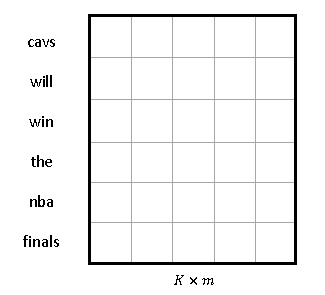
\includegraphics[width=0.55\textwidth]{sentenceMatrix}
  \caption{语句向量化的示意图}
  \label{fig:senVec}
\end{figure}

图\ref{fig:senVec}中每一行表示一个词语向量化得到的一个向量,所有行组成一个语句。在例子中,语句$\mathbf{s}=$\textit{cavs}$\oplus$\textit{will}$\oplus$\textit{win}$\oplus$\textit{the}$\oplus$\textit{NBA}$\oplus$\textit{finals}。语句$\mathbf{s}$中的每一个词语都将根据词向量模型转换成一个向量。这一步骤将语句$\mathbf{s}$转换成一个矩阵$\mathbf{B} \in \mathbb{R}^{Km}$,其中$K$为语句$\mathbf{s}$的长度,$m$为词向量模型设定的维度。对于任意一篇文档$\mathbf{d}_j$,我们能够将其文本摘要,即排序后的语句集合$\mathbf{S}_j = \left\{\mathbf{s}'_1, \mathbf{s}'_2, \cdots, \mathbf{s}'_k\right\}$转换成另一个矩阵$\mathbf{A}_j \in \mathbb{R}^{nm}$,其中$n$为文档长度的截断长度,即允许容纳的最大词语量。我们以图\ref{fig:docVec}为例进行说明。

\begin{figure}[!htbp]
  \centering
  % Requires \usepackage{graphicx}
  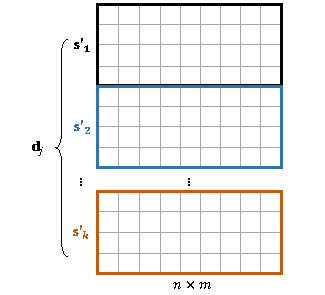
\includegraphics[width=0.65\textwidth]{documentMatrix}
  \caption{文档向量化的示意图}
  \label{fig:docVec}
\end{figure}

图\ref{fig:docVec}为词向量模型将一篇文档$\mathbf{d}_j$转换成矩阵$\mathbf{A}_j$的示意图。如果文档中的长度超过了阈值$n$,则进行截断;如果文档的长度不足$n$,则用零向量进行补全。本小节中的处理过程使得每一篇文档都能转换成一个固定大小的矩阵。但是,在截断或者补全零向量的操作会丢失部分信息或者引用无效的信息,这一问题还是有待今后的工作进行研究。

\subsection{卷积神经网络的训练}
\label{subsec3:cnnTraining}
在上一小节中,我们得到了表示文档的矩阵,我们将此当作输入来训练卷积神经网络。卷积神经网络的框架图如图\ref{fig:cnn}所示。

\begin{figure}[!htbp]
  \centering
  % Requires \usepackage{graphicx}
  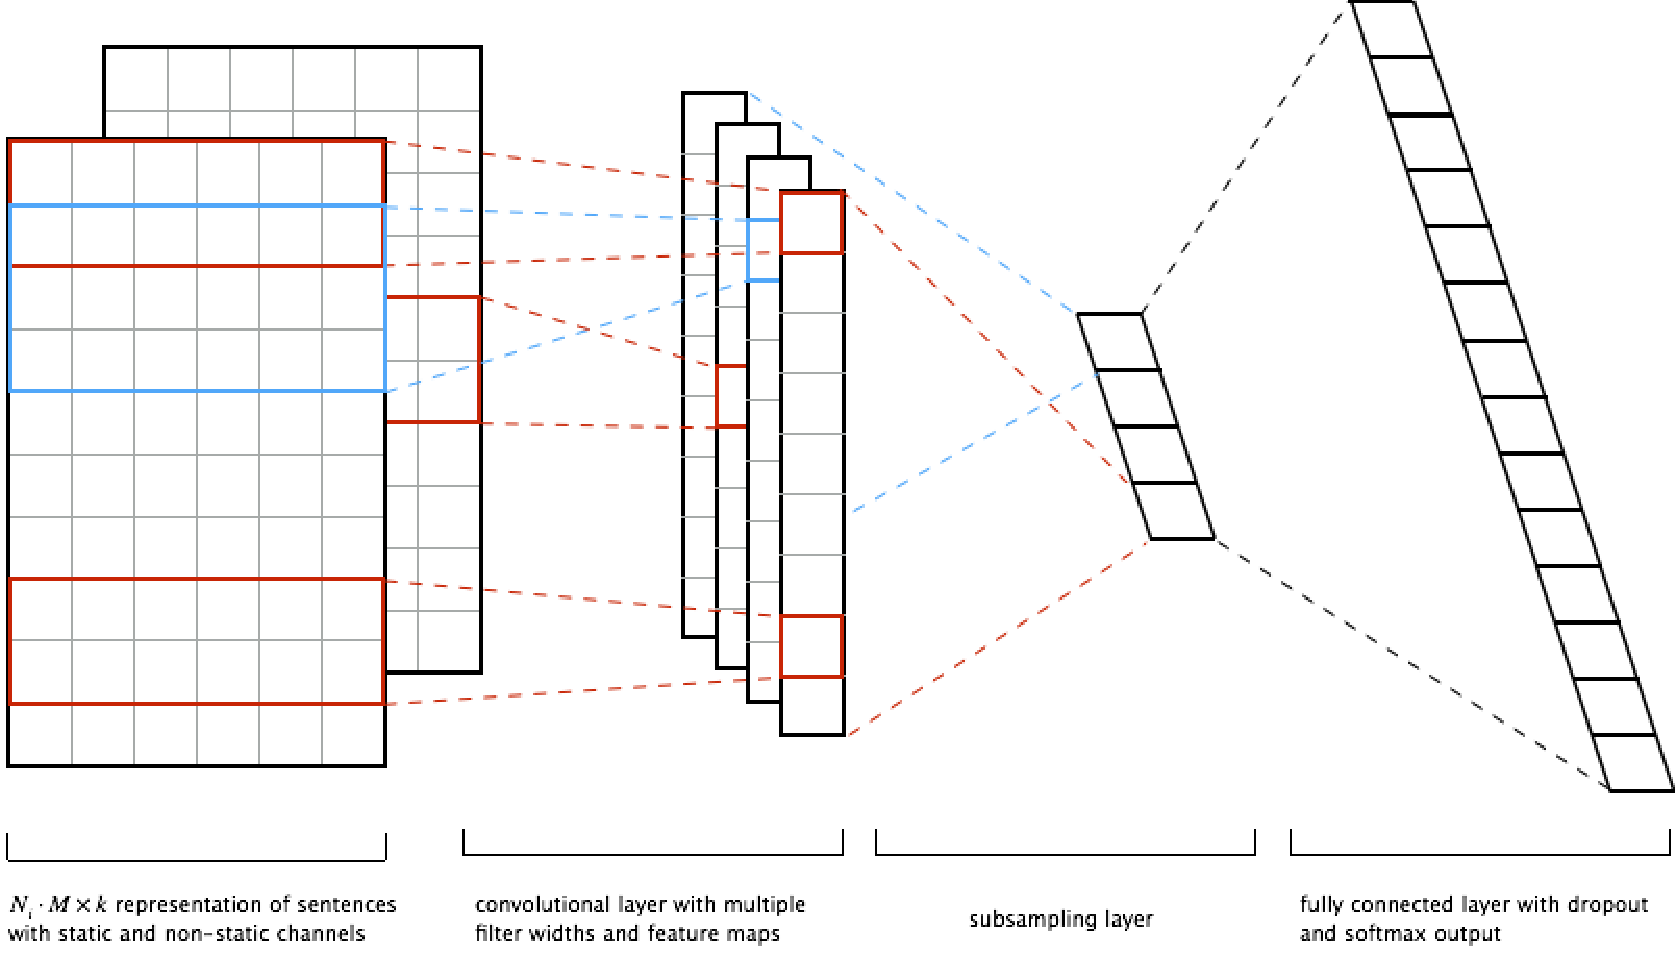
\includegraphics[width=0.85\textwidth]{cnn}
  \caption{三层卷积神经网络结构图}
  \label{fig:cnn}
\end{figure}

图\ref{fig:cnn}中的第一层为卷积层,包含多个宽度的滤波器。我们定义$\mathbf{w} \in \mathbb{R}^{hm}$为卷积层中的一个滤波器,其中$h$为滤波器的窗口大小,即一次性处理词语的窗口大小,$m$为滤波器的宽度,令其等于第\ref{subsec3:word2vec}小节中词向量模型设定的维度。该滤波器作用到一个窗口大小为$h$的文本上,文本中的词语表示成维度为$m$的向量。为了方便起见,我们使用$\mathbf{t}_{i:i+h}$来表示词语$\mathbf{t}_i, \mathbf{t}_{i+1}, \cdots, \mathbf{t}_{i+h}$的连接。一个滤波器$\mathbf{w}$作用到词语连接$\mathbf{t}_{i:i+h}$,将产生一个新的特征$c_i$,可表示成公式(\ref{eq:feature})所示,
\begin{equation}
\label{eq:feature}
	c_i=f(\mathbf{w} \otimes \mathbf{t}_{i:i+h} + b)
\end{equation}
其中$b \in \mathbb{R}$为偏置参数,$f$为一个非线性的函数,例如sigmoid函数等。值得注意的是,在本章中,我们令滤波器$\mathbf{w} \in \mathbb{R}^{hm}$的宽度等于词向量模型的维度。这个步骤与图像处理中的设置不同,这是由于设置一个宽度小于$m$的滤波器在文本处理中是没有意义的。文本中的词语被表示成$m$维的向量,因此截取其中的某些维度是无意义的。对于一篇文档,我们从上至下滑动滤波器,$\mathbf{w} \in \mathbb{R}^{hm}$将作用在不同的词语连接$(\mathbf{t}_{1:h}, \mathbf{t}_{2:h + 1}, \cdots, \mathbf{t}_{N - h + 1:N})$上,从而得到一个新的特征向量$\mathbf{c}$,其可表示为公式(\ref{eq:featureMap})所示,
\begin{equation}
\label{eq:featureMap}
	\mathbf{c}  = ({c_1},{c_2},...,{c_{N - h + 1}})^T
\end{equation}
其中$\mathbf{c} \in \mathbb{R}^{N-h+1}$。在经过卷积层后,得到的特征维数仍然很高,很容易出现过拟合的现象。为了解决这个问题,我们在卷积层后加上一个池化(Pooling)操作,也就是子采样(Subsampling),构成子采样层。子采样层能够大大降低特征的维数,避免过拟合。池化操作作用在特征向量$\mathbf{c}$将得到$\mathbf{c}$中的最大值$c_{\max} = \max\limits_{c_i \in \mathbf{c}} c_i$。子采样层的目的是为了得到特征向量中最为重要的特征值,即具有最大的特征值。为了得到更多的特征值,我们可以调整窗口的大小来产生不同的特征向量。最后,子采样层得到的特征作为最后分类器的输入,该层为一个softmax函数的全连接层,输出层为文档在各个类别上的概率分布。

此外,我们使用了两个通道\upcite{kim2014convolutional}的词向量作为输入。其中一个通道在训练过程中保持不变,另一个通道通过反向传播进行微调。每一个滤波器都会作用于这两个通道来产生不同的特征。

\begin{algorithm}[!ht]
    \caption{\textit{VecCNN}($\mathbf{D}$)}\label{alg:cnn}
    \begin{algorithmic}[1]
    \REQUIRE $\mathbf{D}$
    \ENSURE \textit{CNN}
    \FOR{each $\mathbf{d}_j$ in $\mathbf{D}$}
        \FOR{each $t_i$ in $\mathbf{d}_j$}
            \STATE{${tf}_{ij} = \frac{p_{ij}}{\sum_{tl \in \mathbf{d}_j}{p_{lj}}}$}
            \STATE{${idf}_i = \log \frac{\vert \mathbf{D} \vert}{1 + \vert \{\mathbf{d} \in \mathbf{D} : \mathbf{t}_i \in \mathbf{d}\}\vert}$}
        \ENDFOR
    \ENDFOR
    \FOR{each $\mathbf{d}_j$ in $\mathbf{D}$}
        \FOR{each $\mathbf{s}_i$ in $\mathbf{d}_j$}
            \STATE{$I(\mathbf{s}_i, \mathbf{d}_j)=\frac{\sum \nolimits_{\mathbf{t}_i \in \mathbf{s}_i} {tf}_{ij}\cdot{idf}_i }{\log \left(\vert\mathbf{s}_i\vert\right)}$}
        \ENDFOR
        \STATE{$\mathbf{S}_j = \left\{\mathbf{s}'_1, \mathbf{s}'_2, \cdots, \mathbf{s}'_k\right\}$}
    \ENDFOR
    \FOR{each $\mathbf{S}_j$ in $\mathbf{D}$}
        \STATE{generate text matrix $\mathbf{A}_j$ based on $\mathbf{S}_j$}
    \ENDFOR
    \STATE{train \textit{CNN} based on the matrix set}
    \STATE {\textbf{return:} \textit{CNN}}
    \end{algorithmic}
\end{algorithm}

本节中的算法步骤可以概括为算法\ref{alg:cnn}所示。如算法VecCNN算法所示,输入为已标注的长文本信息集合,即文档集合$\mathbf{D}$,输出为所设计的卷积神经网络各层的参数。算法中的第1行至第6行为词语的tf-idf值计算。在这个步骤中,我们计算了每一个文档中各个词语的tf-idf值,为之后的文本摘要提取做准备。算法中的第7行至第12行,我们根据语句中词语的tf-idf值来对文档中的语句进行排序,从而挑选出关键语句代表文档的主题。这个过程减少了输入文本信息的规模,方便了之后卷积神经网络的训练。算法的第13行至第17行是卷积神经网络的训练。我们选择top-$k$的语句构建矩阵,作为卷积神经网络的输入,计算各个神经元中参数的梯度,通过迭代的方法求得极值,训练得到网络各层的参数。


\section{实验分析}
\label{sec3:experiment}

\section{本章小结}
\label{sec3:conclusion}